\section{Proposed Framework}
\label{sec:proposed_method}

\begin{figure*}[t]
    \centering
    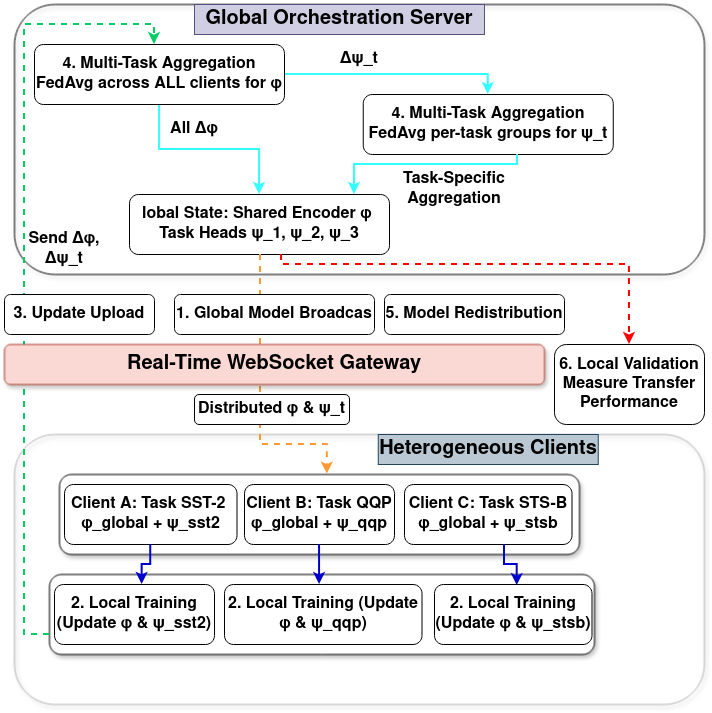
\includegraphics[width=0.85\textwidth]{plots/FL_MTL_FRAME_WORK.png}
    \caption{Architecture of the developed framework for real-time federated MTL.}
    \label{fig:framework_pipeline}
\end{figure*}

The proposed RT-FedMTL simultaneously addresses the challenges of balancing privacy-preserving NLU and resource-constrained edge computing. We introduce a modular federated-based architecture tailored for real-time asynchronous synchronization across WebSockets, multi-task learning (leveraging common linguistic representations with task-specific specialization), and parameter-efficient SLMs to reduce the computational and communication footprint on edge devices.

\subsection{System Overview}
As illustrated in Fig.~\ref{fig:framework_pipeline}, a high level orchestration server, and several heterogeneous client nodes form the basis of the architecture. A parameter server maintains a global state at the center and controls the model aggregation logic. The communications depend on low-latency WebSockets for a bidirectional exchange of model updates, and aggregated parameters.


Federated components and privacy constraints of a system are built on:
\begin{itemize}
    \item Global server $\mathcal{S}$: orchestrates client sampling, model broadcast, and aggregation.
    \item Distributed clients $\mathcal{C}$: edge devices/silos to store the raw text.
    \item Functional modules ($f_e, h_k$): the shared backbone and task-specific heads parameterized by $\theta_e, \theta_k$ (see Fig.~\ref{fig:framework_pipeline}).
    \item Local datasets $\mathcal{D}_c^t$: private data streams for the client $c$ at round $t$.
\end{itemize}

For the sake of privacy, samples are never uploaded. Each of these clients sends only model updates (or compressed adapter and head updates) and acts as host-side aggregation \cite{mcmahan2017communication,elbakary2025mira}. This is in line with the traditional federated privacy model in which data locality is retained and collaborative training is advocated in the field.

\subsection{Backbone of Small Language Model (SLMs)} This approach enables special SLMs for ensuring an optimal computational efficiency with high language understanding. We use architectures such as DistilBERT \cite{sanh2019distilbert}, BERT-Medium \cite{turc2019well}, MiniLM \cite{wang2020minilm} for resource-constrained environments. The SLM backbone consists of several integral stages:

\subsubsection{Tokenizer and Embedding Layer} Outputs are inputted and processed by input text subword tokenizer that converts raw strings into a series of tokens. The generated tokens map to a high-dimensional vector space by means of a learned embedding layer. To model sequence structures without the overhead of recurrences, we add learnable position embeddings at the level of the token embeddings providing the machine with necessary context about the order of the tokens.

\subsubsection{Low-Cost Transformer Encoder} The central element is a lightweight transformer encoder. These models consist of fewer layers and smaller hidden dimensionality than traditional BERT-base architectures \cite{devlin2019bert}. Each layer utilizes multi-head self-attention for long-range dependencies and the feed-forward network for feature transformation. This streamlined way significantly reduces parameter number and computational load, thus allowing for fast inference and training on edge devices.

\subsubsection{Shared Representation} The encoder generates a dense vector, represented as a shared representation $f_e(x; \theta_e)$. This captures the basic semantically and syntactically fundamental information in the input. In our multi-task framework, with the backbone shared across all tasks the model learns universal linguistic patterns while task specific heads focus on unique output. This federated learning-based collaborative tuning guarantees strong generalization across heterogeneous client data.

\subsection{Multi-Task Learning Strategy}
We adopt a hybrid approach of sharing the parameters. Throughout the tasks that all share linguistic representation, the lower (encoder) layers of the transformer remains unchanged. On the other hand, top layers are task-centric classification or regression heads respectively. We thus maintain an adaptive loss weighting mechanism to minimize negative transfer:
\begin{equation} \label{eq:total_multi_task_loss}
    \mathcal{L}_{total} = \sum_{j=1}^{K} w_j \mathcal{L}_j
\end{equation}
where $w_j$ are task weights dynamically tuned for each task $j$ based on the convergence rate. This formulation ensures that the local update step in Algorithm~\ref{alg:rt_fedmtl} minimizes the regularized objective function defined in Eq. \eqref{eq:universal_goal}.

We define the parameters
\begin{equation} \label{eq:parameter_set}
    \Theta = \{\theta_e, \{\theta_k\}_{k=1}^{K}\},
\end{equation}
where $\theta_e$ parameterizes the SLM encoder $f_e$ and $\theta_k$ parameterizes the task head $h_k$ for task $k$ \cite{chen2024fedbone,zhou2025multi}. Prediction for input $x$ in task $k$ is given by:
\begin{equation} \label{eq:prediction_head}
    \hat{y} = h_k\big(f_e(x;\theta_e);\theta_k\big),
\end{equation}
where $f_e(\cdot)$ and $h_k(\cdot)$ represent the components optimized in Algorithm~\ref{alg:rt_fedmtl} to maximize sharing while preserving task-specificity.

\subsection{Federated Optimization and Real-Time Adaptation}
The federated optimization process is described in Algorithm~\ref{alg:rt_fedmtl}. This system enables real-time adaptation by dynamically synchronizing updates on request via WebSockets. Using a task-aware version of FedAvg \cite{mcmahan2017communication}, the server aggregates updates and normalizes noise from heterogeneous sources (non-IID). Most recent work in adaptive federated optimization \cite{reddi2020adaptive} suggests incorporating momentum and adaptive learning rates will add an even greater level of stability.

\begin{algorithm}
\caption{RT-FedMTL: Real-time federated MTL}
\label{alg:rt_fedmtl}
\begin{algorithmic}[1]
\STATE Server Initialize: Shared encoder $\theta_{e,0}$, task heads $\{\theta_{j,0}\}_{j=1}^K$
\FOR{each round $t = 1, 2, \dots$}
    \STATE Server broadcasts $\theta_{e,t}, \theta_{Task(c),t}$ (for $f_e, h_k$) to clients $c \in \mathcal{C}_t$
    \FOR{each client $c \in \mathcal{C}_t$ in parallel}
        \STATE Local training: $\{\theta_{e,c}^{t+1}, \theta_{Task(c),c}^{t+1}\} \leftarrow \text{LocalUpdate}(\mathcal{D}_c, f_e, h_k, \theta_{e,t}, \theta_{Task(c),t})$ \COMMENT{Optimize $h_k(f_e(\cdot))$}
        \STATE Updates $\{\theta_{e,c}^{t+1}, \theta_{Task(c),c}^{t+1}\}$ via WebSockets to Server
    \ENDFOR
    \STATE Encoder Aggregation:
    \STATE \quad $\theta_{e,t+1} \leftarrow \sum_{c\in\mathcal{C}_t} \alpha_c^t \theta_{e,c}^{t+1}$ \COMMENT{Aggregate shared backbone $f_e$}
    \FOR{each task $k \in \{1,\dots,K\}$ in parallel}
        \STATE $\theta_{k,t+1} \leftarrow \sum_{c \in\mathcal{C}_t: \, \tau(c)=k} \beta_c^t \theta_{k,c}^{t+1}$ \COMMENT{Aggregate specialized head $h_k$}
    \ENDFOR
    \STATE Server assigns $\{\theta_{e,t+1}, \theta_{Task(c),t+1}\}$ for Local Validation
\ENDFOR
\end{algorithmic}
\end{algorithm}

\subsection{Communication-Efficient Fine-Tuning}
To further reduce resource usage in edge devices, we perform low-rank adaptation (LoRA) \cite{hu2022lora}. This ranges from updating in local $B$, where instead of updating the full weight matrices $W \in \mathbb{R}^{d \times d}$, we optimize the low rank decomposition matrices $A$ and $B$, where:
\begin{equation} \label{eq:lora_decomposition}
    W' = W + \Delta W = W + BA.
\end{equation}
$A \in \mathbb{R}^{r \times d}$ and $B \in \mathbb{R}^{d \times r}$ with rank $r \ll d$. When performing big updates, only the matrices $A$ and $B$ are sent, minimizing communication volume up to 99\%.